\documentclass[conference]{IEEEtran}

\usepackage{amsmath}
\usepackage{booktabs}
\usepackage{graphicx}
\usepackage{url}

\title{Stochastic Optimization of Airbag Deployment Parameters Under Crash Uncertainty}

\author{
\IEEEauthorblockN{Jaladhi Joshi (22B0994) and Manav Agrawal (22B1253)}
\IEEEauthorblockA{ME 701 Course Project}
}

\begin{document}
\maketitle

\begin{abstract}
Airbag deployment must be robust to uncertainty in crash speed, impact angle, occupant position, belt usage, and sensor timing. This project formulates deployment tuning as a stochastic constrained optimization problem. A reduced-order occupant-restraint simulator is used to evaluate candidate deployment designs over Monte Carlo crash scenarios. The optimized design variables are trigger delay, early pressure, mid pressure, late pressure, and vent rate. The objective combines mean head injury criterion (HIC), chest deflection, deployment energy, HIC tail risk through CVaR, HIC failure probability, and false deployment probability. We compare a reference design, deterministic SQP, grid search, an MPC-inspired adaptive policy, robust Differential Evolution with SLSQP refinement, a shift-robust DRO-style optimizer, and shift-refined local search. In the selected final run, shift-refined local search reduced shifted-distribution mean HIC from 444.16 to 372.21 and reduced HIC failure rate from 32.00\% to 20.33\% relative to the initial design.
\end{abstract}

\begin{IEEEkeywords}
airbag deployment, stochastic optimization, robust design, crash safety, HIC, CVaR, distribution shift
\end{IEEEkeywords}

\section{Introduction}
Airbag deployment is a timing and force-management problem under uncertainty. A deployment setting that is reasonable for a nominal frontal crash may not remain safe when impact speed, obliquity, occupant offset, belt usage, or sensor delay changes. Therefore, a robust deployment design should be evaluated over a distribution of crash scenarios rather than a single prescribed case.

The objective of this project is to build a reproducible computational workflow for comparing airbag deployment optimization methods. The simulator is intentionally reduced order, so the numerical results should be interpreted as algorithmic comparisons rather than as certified crash-safety predictions. Within this simplified setting, the main question is: which optimization method produces deployment parameters that reduce both average injury and high-risk tail outcomes?

\section{Problem Formulation}
The deployment design vector is
\begin{equation}
x = [d, p_e, p_m, p_l, v]^T,
\end{equation}
where $d$ is trigger delay in ms, $p_e$, $p_m$, and $p_l$ are early, middle, and late inflation pressure levels in kPa, and $v$ is the vent rate.

A random crash scenario is denoted by
\begin{equation}
\xi = [s, \theta, o, b, \tau_s, T_p, a_b]^T,
\end{equation}
where $s$ is crash speed, $\theta$ is impact angle, $o$ is occupant offset, $b$ is belt usage, $\tau_s$ is sensor delay, $T_p$ is crash pulse duration, and $a_b$ is trigger acceleration bias. For each pair $(x,\xi)$, the simulator returns
\begin{equation}
y(x,\xi)=\{\mathrm{HIC},D_c,E,I_f,I_{fd}\},
\end{equation}
where $D_c$ is chest deflection, $E$ is deployment energy, $I_f$ indicates injury failure, and $I_{fd}$ indicates false deployment.

The design goal is to reduce injury metrics while limiting excessive energy and false deployment. The project uses a sample-average approximation because the objective cannot be evaluated analytically.

\section{Mathematical Model}
Let $\{\xi_i\}_{i=1}^{N}$ be sampled crash scenarios. For a fixed design $x$, define
\begin{align}
\overline{H}(x) &= \frac{1}{N}\sum_{i=1}^{N}\mathrm{HIC}(x,\xi_i),\\
\overline{D}(x) &= \frac{1}{N}\sum_{i=1}^{N}D_c(x,\xi_i),\\
\overline{E}(x) &= \frac{1}{N}\sum_{i=1}^{N}E(x,\xi_i).
\end{align}
The empirical HIC failure and false deployment probabilities are
\begin{align}
\hat{p}_f(x) &= \frac{1}{N}\sum_{i=1}^{N}\mathbf{1}\{\mathrm{HIC}(x,\xi_i)>H_{\max}\},\\
\hat{p}_{fd}(x) &= \frac{1}{N}\sum_{i=1}^{N}I_{fd}(x,\xi_i).
\end{align}
The implemented HIC threshold is $H_{\max}=500$ in the optimizer configuration, while report tables also show the severe-event failure behavior generated by the model.

Tail risk is measured with empirical CVaR at confidence level $\alpha=0.90$:
\begin{equation}
\mathrm{CVaR}_{0.90}(H)=
\frac{1}{|\mathcal{T}|}\sum_{i\in \mathcal{T}}\mathrm{HIC}(x,\xi_i),
\end{equation}
where $\mathcal{T}=\{i:\mathrm{HIC}(x,\xi_i)\geq q_{0.90}\}$ and $q_{0.90}$ is the empirical 90th percentile of HIC.

The simulation-based optimization problem is
\begin{align}
\min_{x\in\mathcal{X}} J(x)=
&\;0.55\frac{\overline{H}(x)}{1000}
+0.25\frac{\overline{D}(x)}{60}
+0.08\overline{E}(x) \nonumber\\
&+0.12\frac{\mathrm{CVaR}_{0.90}(H)}{1200}
+0.20\hat{p}_{fd}(x) \nonumber\\
&+6\max(0,\hat{p}_f(x)-0.10)^2 \nonumber\\
&+10\max(0,\hat{p}_{fd}(x)-0.02)^2 \nonumber\\
&+2\frac{\max(0,\overline{D}(x)-55)^2}{55^2}.
\end{align}
The feasible set is
\begin{align}
\mathcal{X}= \{x:\;&5\leq d\leq40,\quad
100\leq p_e,p_m,p_l\leq300,\nonumber\\
&4\leq v\leq45\}.
\end{align}
The normalizing constants in $J(x)$ put HIC, chest deflection, CVaR, and energy on comparable scales. The squared penalties discourage designs that look good on average but violate chance-style safety targets.

\section{Scenario Sampling and Simulation}
Crash scenarios are sampled from two profiles. The default profile is used for nominal stochastic training and in-distribution evaluation. The shifted profile increases severity by sampling higher speeds, larger impact angles, larger occupant offsets, lower belt-use probability, and noisier sensor delay.

For active crashes, speed is sampled from a beta distribution mapped to 30--60 mph:
\begin{equation}
s = s_{\min} + (s_{\max}-s_{\min})U_s,\quad U_s\sim \mathrm{Beta}(a_s,b_s).
\end{equation}
The shifted profile changes the beta parameters to move probability mass toward higher speeds. Impact angle is sampled by multiplying a beta-distributed magnitude by a random sign. Sensor delay is generated using a discrete Ornstein-Uhlenbeck style process,
\begin{equation}
z_{k+1}=\phi z_k+\sigma\epsilon_k,\quad \epsilon_k\sim\mathcal{N}(0,1),
\end{equation}
and then clipped to a physically reasonable delay range.

The simulator uses one-dimensional occupant forward motion with belt slack, belt stiffness and damping, pretensioner action, airbag pressure build-up, venting, airbag contact, and hard-stop contact. The head acceleration signal is filtered and used to compute a HIC-style proxy over a 36 ms window. The chest deflection proxy is computed from belt, airbag, and hard-stop force response.

\section{Optimization Methods}
This section gives the methodology and mathematics of each method.

\subsection{Initial Reference Design}
The initial design is not optimized. It is a fixed reference vector
\begin{equation}
x_0=[18,\;220,\;190,\;140,\;18]^T.
\end{equation}
All improvement percentages are computed relative to this baseline. It is included so that every optimizer can be compared against the same starting point.

\subsection{Deterministic SQP}
The deterministic SQP baseline solves a single-scenario optimization problem:
\begin{equation}
x_{\mathrm{SQP}}=\arg\min_{x\in\mathcal{X}}J_{\mathrm{nom}}(x;\xi_{\mathrm{nom}}).
\end{equation}
The nominal scenario is a 45 mph, zero-angle, belted crash with no occupant offset, no sensor delay, and nominal pulse duration. The objective $J_{\mathrm{nom}}$ uses the same metric formula as the stochastic objective, but with $N=1$.

This method is included because it represents a common nominal engineering workflow: choose one design case and optimize locally. SLSQP is appropriate here because the problem has smooth bound constraints and a small number of continuous variables. Its weakness is that it ignores scenario variation, so it can produce a design that does not reduce distribution-level risk.

\subsection{Coarse Grid Search with Refinement}
Grid search evaluates a finite candidate set:
\begin{equation}
\mathcal{G}=\mathcal{D}\times\mathcal{P}_e\times\mathcal{P}_m\times\mathcal{P}_l\times\mathcal{V}.
\end{equation}
The implemented coarse grids are
\begin{align}
\mathcal{D}&=\{6,16,28,38\},\\
\mathcal{P}_e&=\{100,170,240,300\},\\
\mathcal{P}_m&=\{160,220,270,300\},\\
\mathcal{P}_l&=\{100,160,210,260\},\\
\mathcal{V}&=\{4,12,24,45\}.
\end{align}
The selected grid design is
\begin{equation}
x_{\mathrm{grid}}=\arg\min_{x\in\mathcal{G}}\hat{J}_{24}(x),
\end{equation}
where $\hat{J}_{24}$ evaluates the objective on the first 24 stochastic training scenarios for computational efficiency. After the coarse pass, a local grid is built around the best candidate to refine the result.

Grid search is included because it is transparent and does not depend on gradients. It is computationally expensive in higher dimensions, but with five variables and a coarse grid it gives a useful sanity check for the more sophisticated optimizers.

\subsection{MPC-Inspired Adaptive Policy}
The MPC-inspired method is not a fixed design. It maps each observed scenario to a design:
\begin{equation}
x_i=\pi(\xi_i).
\end{equation}
The policy first computes normalized severity features:
\begin{align}
r_s &= \mathrm{clip}\left(\frac{s-30}{30},0,1\right),\\
r_\theta &= \mathrm{clip}\left(\frac{|\theta|}{35},0,1\right),\\
r_o &= \mathrm{clip}\left(\frac{o+0.06}{0.13},0,1\right).
\end{align}
It then forms a scalar severity score
\begin{equation}
\rho=\mathrm{clip}(0.62r_s+0.18r_\theta+0.10r_o+\delta_b,0,1),
\end{equation}
where $\delta_b=0.18$ if the occupant is unbelted and $0$ otherwise.

The policy computes deployment variables as affine functions of severity:
\begin{align}
d &= 24-16\rho-500\tau_s,\\
p_e &= 115+55\rho+15r_\theta,\\
p_m &= 205+95\rho+10r_o,\\
p_l &= 135+60\rho+10r_\theta,\\
v &= 28-18\rho+4r_\theta.
\end{align}
Each value is clipped to the feasible bounds. This method is included as a simple adaptive-control baseline. It mimics the idea of changing deployment aggressiveness based on sensed crash severity, without solving a full online optimal-control problem.

\subsection{Robust DE+SLSQP}
The main robust optimizer solves the sample-average stochastic problem
\begin{equation}
x_{\mathrm{rob}}=\arg\min_{x\in\mathcal{X}}\hat{J}_{N_{\mathrm{train}}}(x),
\end{equation}
where $N_{\mathrm{train}}=500$ default-profile scenarios. The method has two stages.

First, Differential Evolution searches globally over $\mathcal{X}$. In general form, candidate vectors are mutated using
\begin{equation}
u = x_a + F(x_b-x_c),
\end{equation}
followed by crossover and selection based on objective value. This helps explore nonconvex regions of the design space without requiring gradients.

Second, SLSQP starts from the best global candidate and performs local constrained refinement:
\begin{equation}
x^{k+1}=x^k+\Delta x^k,
\end{equation}
where $\Delta x^k$ is computed from a local sequential quadratic programming approximation while respecting the bounds. This global-then-local structure is used because the objective is simulation-based and may contain multiple local minima.

\subsection{Shift-Robust DRO-Style Optimization}
The shift-robust method is designed to reduce sensitivity to distribution mismatch. Instead of relying only on default training scenarios, it gives attention to shifted scenarios. Conceptually, the objective can be written as
\begin{equation}
J_{\mathrm{shift}}(x)=
(1-\eta)\hat{J}_{\mathrm{default}}(x)
+\eta\hat{J}_{\mathrm{shifted}}(x),
\end{equation}
with $\eta>0$ increasing emphasis on severe shifted cases. This is a simplified distributionally robust idea: the design should perform well not only under the nominal distribution but also under a nearby or more severe evaluation distribution.

This method is included to test whether explicitly training against shifted cases improves out-of-distribution performance.

\subsection{Shift-Refined Local Search}
Shift-refined local search starts from the robust fixed design and performs a focused coordinate-pattern refinement using additional shifted scenarios. The optimization target is
\begin{equation}
x_{\mathrm{ref}}=\arg\min_{x\in\mathcal{N}(x_{\mathrm{rob}})\cap\mathcal{X}}
\hat{J}_{\mathrm{shift-ref}}(x),
\end{equation}
where $\mathcal{N}(x_{\mathrm{rob}})$ is a local neighborhood around the robust design. Multiple seed candidates are generated from the robust solution, and each seed is refined by testing positive and negative coordinate steps. If a candidate improves the objective, it becomes the new center of the local search; otherwise the step size is reduced.

This method is included because the robust optimizer improved shifted performance but did not directly target the most severe shifted evaluation profile. Local shifted refinement is computationally cheaper than a full new global search and can correct remaining distribution-shift weaknesses.

\section{Experimental Setup}
The experiment uses a fixed random seed for reproducibility. The workflow samples 500 default training scenarios, 300 shifted training scenarios, and 3000 evaluation scenarios for each profile. Every fixed design is evaluated on the same evaluation scenarios, which makes method comparisons fair.

The final selected result bundle is \texttt{outputs/03\_domain\_shift\_run}. It contains scenario-level metrics, comparison tables, design tables, method summaries, trace plots, histograms, boxplots, and tradeoff plots.

\section{Results}
Table~\ref{tab:iid} summarizes in-distribution evaluation. Table~\ref{tab:shifted} summarizes shifted-distribution evaluation.

\begin{table}[!t]
\caption{In-Distribution Evaluation}
\label{tab:iid}
\centering
\begin{tabular}{lccc}
\toprule
Method & Obj. & Mean HIC & Fail. \%\\
\midrule
Initial & 0.431 & 259.89 & 16.00\\
Deterministic SQP & 0.431 & 259.85 & 16.00\\
Grid Search & 0.379 & 249.09 & 14.33\\
MPC-Inspired & 0.415 & 247.59 & 12.67\\
Robust DE+SLSQP & 0.356 & 230.41 & 11.67\\
Shift-Robust DRO & 0.367 & 238.52 & 12.67\\
Shift-Refined & \textbf{0.352} & \textbf{226.52} & \textbf{11.00}\\
\bottomrule
\end{tabular}
\end{table}

\begin{table}[!t]
\caption{Shifted-Distribution Evaluation}
\label{tab:shifted}
\centering
\begin{tabular}{lccc}
\toprule
Method & Obj. & Mean HIC & Fail. \%\\
\midrule
Initial & 0.892 & 444.16 & 32.00\\
Deterministic SQP & 0.891 & 443.96 & 32.00\\
Grid Search & 0.738 & 401.87 & 28.67\\
MPC-Inspired & 0.766 & 412.99 & 27.33\\
Robust DE+SLSQP & 0.589 & 377.17 & 21.00\\
Shift-Robust DRO & 0.658 & 386.90 & 25.00\\
Shift-Refined & \textbf{0.579} & \textbf{372.21} & \textbf{20.33}\\
\bottomrule
\end{tabular}
\end{table}

\begin{table}[!t]
\caption{Best Shift-Refined Fixed Design}
\label{tab:design}
\centering
\begin{tabular}{lc}
\toprule
Variable & Value\\
\midrule
Trigger delay & 25.39 ms\\
Early pressure & 300.00 kPa\\
Mid pressure & 300.00 kPa\\
Late pressure & 120.73 kPa\\
Vent rate & 4.00\\
\bottomrule
\end{tabular}
\end{table}

The deterministic SQP solution is almost identical to the initial design, which confirms that nominal optimization is not enough for this uncertainty-heavy problem. Grid search improves both distributions, demonstrating that pressure and venting changes matter. Robust DE+SLSQP improves further by optimizing over many stochastic scenarios. Shift-refined local search performs best on both profiles, reducing shifted mean HIC by 16.2\% and shifted failure rate by 36.5\% relative to the initial design.

\begin{figure}[!t]
\centering
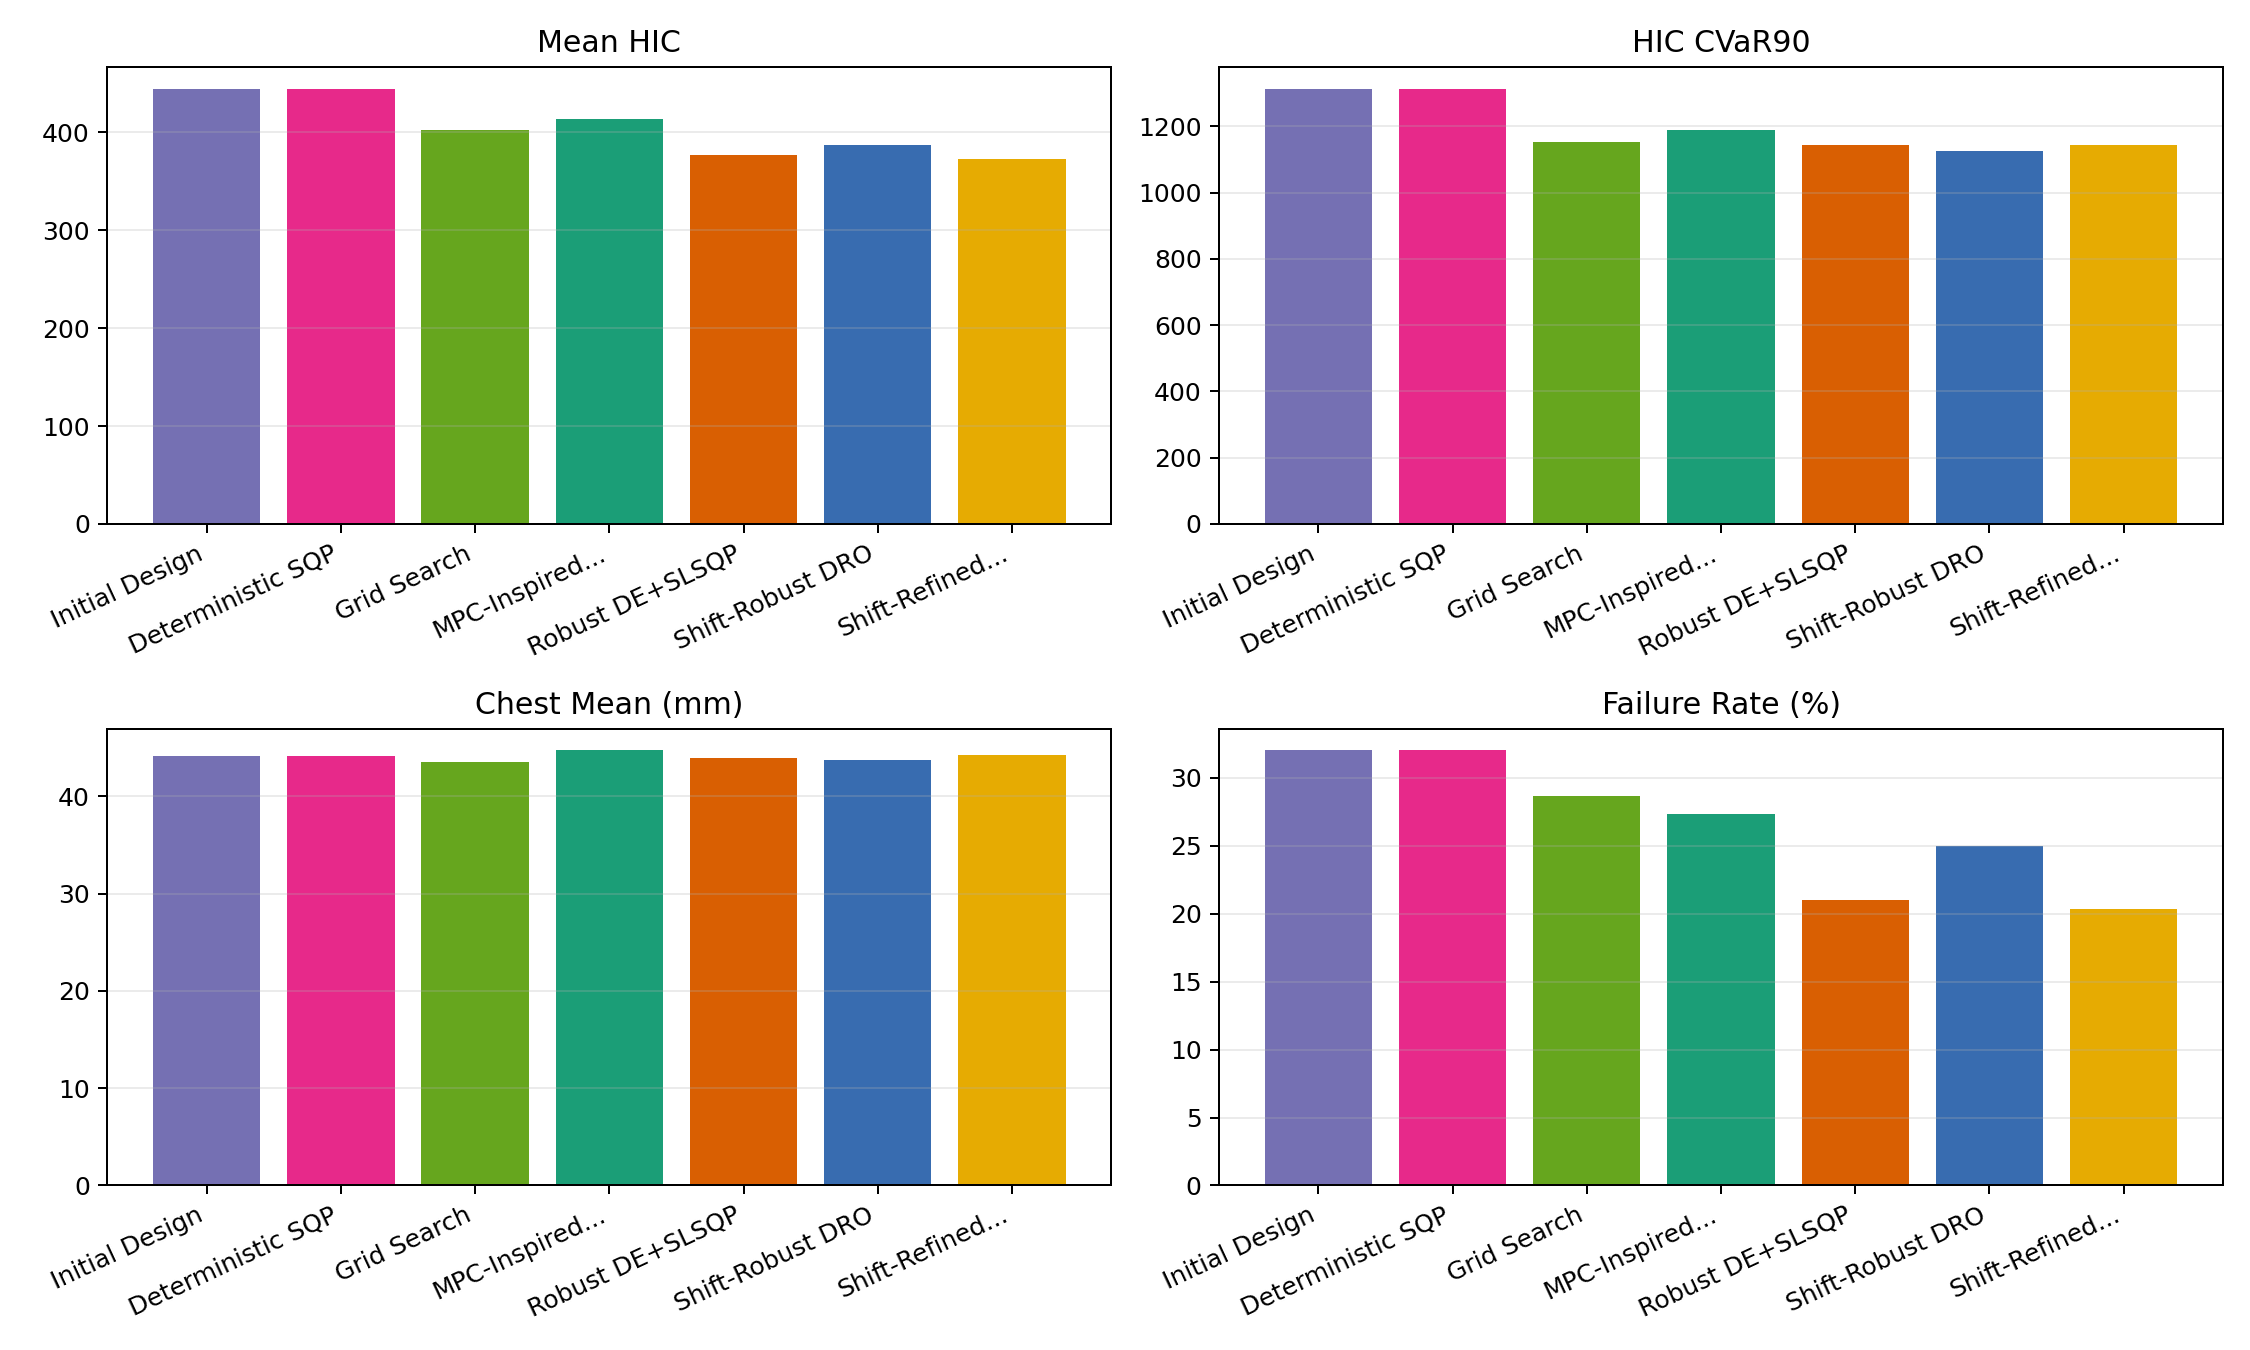
\includegraphics[width=\linewidth]{figures/02_shifted_method_comparison.png}
\caption{Method comparison under shifted evaluation.}
\label{fig:shifted-comparison}
\end{figure}

\begin{figure}[!t]
\centering
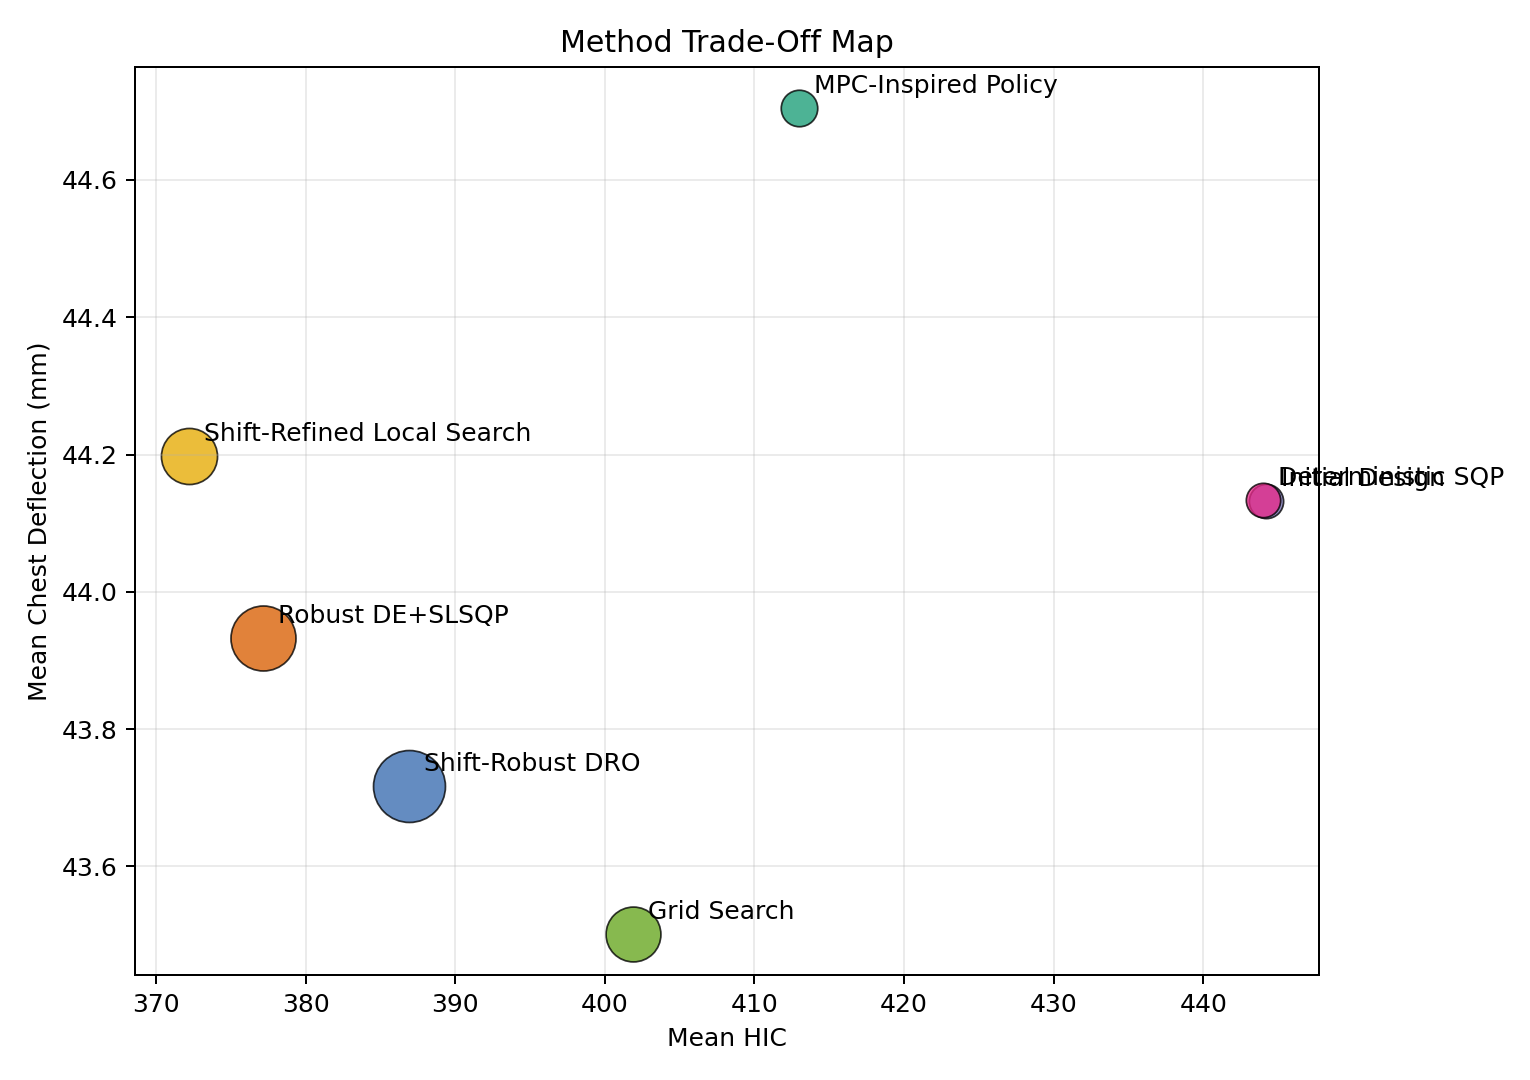
\includegraphics[width=\linewidth]{figures/02_shifted_tradeoff_map.png}
\caption{Tradeoff between injury and energy metrics for shifted evaluation.}
\label{fig:tradeoff}
\end{figure}

\section{Discussion}
The best designs tend to use high early and mid pressure with low venting. In the reduced-order model, this creates stronger early restraint and reduces high-HIC tail outcomes. The late pressure is not simply maximized, which suggests that pressure timing matters as well as total pressure magnitude.

The shifted evaluation is the more important robustness test. The initial design degrades strongly under shift, while the stochastic methods remain more stable. The robust method reduces shifted objective from 0.892 to 0.589, and the shift-refined method improves it further to 0.579. This supports the main hypothesis that deployment tuning should explicitly include uncertainty and distribution shift.

\section{Limitations}
The simulator is intentionally simplified. It does not include a validated finite-element vehicle model, a multibody occupant model, detailed airbag fabric dynamics, real accident database calibration, occupant anthropometry variation, or full side-impact geometry. HIC and chest deflection are proxy metrics, not certified regulatory outputs. The shifted distribution is designed for algorithm testing and is not a statistically validated real-world crash distribution. Therefore, the results should be interpreted as optimization-method comparisons within the project simulator, not as real-world airbag safety certification.

\section{Conclusion}
This project shows that stochastic and shift-aware optimization can substantially improve airbag deployment parameters in a reduced-order crash model. The final shift-refined design outperforms nominal and baseline methods on both default and shifted evaluation scenarios. The main technical lesson is that robustness to uncertainty and distribution shift should be treated as a central part of restraint-system design rather than as an afterthought after nominal tuning.

\section*{Reproducibility}
The code entry point is \texttt{3\_Code/src/run\_experiment.py}. Running the script regenerates numbered output folders containing comparison tables, design tables, scenario-level metrics, and figures. The final selected outputs used in this report are included in \texttt{4\_Data\_Results/outputs/}.

\begin{thebibliography}{1}
\bibitem{storn}
R. Storn and K. Price, ``Differential evolution--a simple and efficient heuristic for global optimization over continuous spaces,'' \emph{Journal of Global Optimization}, 1997.
\bibitem{rockafellar}
R. T. Rockafellar and S. Uryasev, ``Optimization of conditional value-at-risk,'' \emph{Journal of Risk}, 2000.
\bibitem{nhtsa}
NHTSA, ``Development of improved injury criteria for the assessment of advanced automotive restraint systems,'' 1999.
\bibitem{bental}
A. Ben-Tal, L. El Ghaoui, and A. Nemirovski, \emph{Robust Optimization}. Princeton University Press, 2009.
\end{thebibliography}

\end{document}
